\subsection{Ballmaschine}
\begin{tabular}{p{3.6cm}p{9.4cm}}
\rule{0pt}{11pt}\textit{Typ}              & Ballmaschine \\ 
\rule{0pt}{11pt}\textit{Datum}:           & 18.10.2014   \\
\rule{0pt}{11pt}\textit{Ort}:             & Labor HSLU \\
\rule{0pt}{11pt}\textit{Tester}:          & Gruppe 32 \\
\rule{0pt}{11pt}\textit{Ziel des Testes}: & Das Ziel dieses Testes 
bestand darin, den gebauten Prototyp (Ballmaschine) auf die Genauigkeit 
und Wurfweite zu testen, weitere Erkenntnisse über die Drehzahl der Räder 
zu eruieren und die erforderliche Stromstärke unter realen Bedingungen 
testen.  \\
\rule{0pt}{11pt}\textit{Fazit / Verbesserungs-\newline vorschlag}: & 
Die Wurfmaschine kann mit einigen Verbesserungen sehr gute und genaue 
\enquote{Schüsse} erzielen. Zu verbessern sind:
\begin{itemize}
    \item Stabilere Achsen
    \item genauere und gleichmässige Zuführung der Bälle.
    \item einstellbares Grundgerüst
\end{itemize}\\
\end{tabular}

Der Wurfmechanismus besteht aus zwei Kunststoffrädern mit einer weichen 
Pneubeschichtung. Die Räder sind an einer Metallplatte, direkt auf der 
Welle der Motoren angebracht. Die Motoren sind zwei Gleichstrommotoren, 
welche direkt an ein Netzteil angeschlossen sind. Die Drehzahl wird 
über die Spannungsstärke geregelt. Der Abwurfwinkel ist durch die Stellung 
der Metallplatte gegeben, welche in einem beweglichen Schraubstock 
eingespannt ist. Dadurch können diverese Winkel eingestellt werden. 
Die Zuführung der Bälle erfolgt manuell über eine Schiene.
\begin{figure}[h!]
	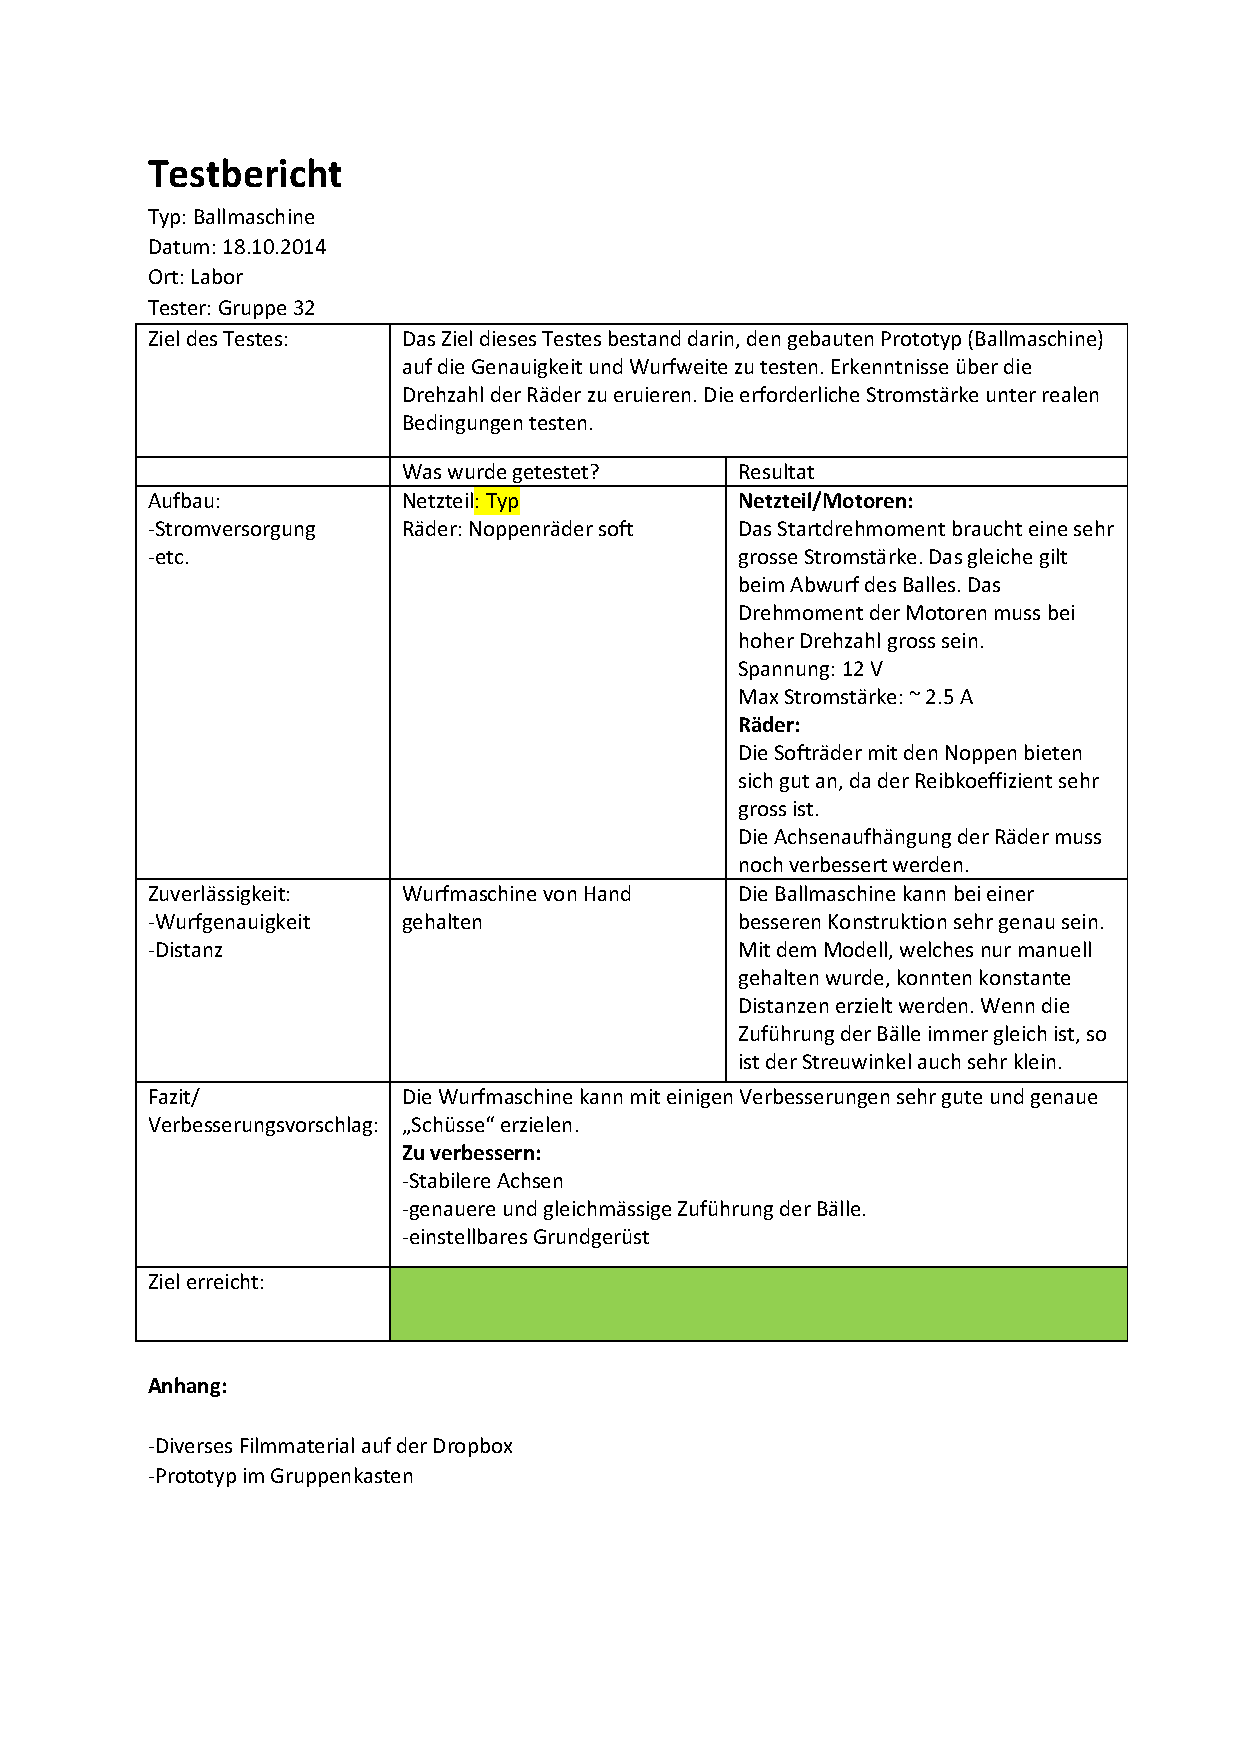
\includegraphics[width=0.77\textwidth,clip,trim=0mm 0cm 0mm 0cm]
	{Funktionstests/Bilder/Ballmaschine.jpg}
	\centering
	\caption{Funktionsmuster Ballmaschine} 
    \label{abb:Ballmaschine_Drehzahl}
\end{figure}